\documentclass[12pt, a4paper, twoside]{article}

%% Preamble
\usepackage{pdfpages}           % Para incluir PDFs
\usepackage{graphicx}           % Para gráficos
\usepackage{subfiles}           % Para manejar subarchivos
\usepackage{hyperref}           % Para enlaces
\usepackage{listings}           % Para código fuente (ajusta lenguaje)
\usepackage{verbatim}
\usepackage[backend=bibtex,style=numeric]{biblatex} % Para citas numéricas
\addbibresource{references.bib} % Cargar archivo .bib
\usepackage{url}


\usepackage{geometry}           % Para ajustar márgenes

% Ajustes de márgenes
\geometry{
	left=3cm,       % Margen izquierdo
	right=3cm,      % Margen derecho
	top=2.5cm,      % Margen superior
	bottom=2.5cm,   % Margen inferior
	headheight=15pt, % Altura del encabezado
	twoside          % Para documentos a dos caras
}


\graphicspath{{images/}{../images/}} % Ruta para imágenes

\begin{document}
	
	%% Cover
	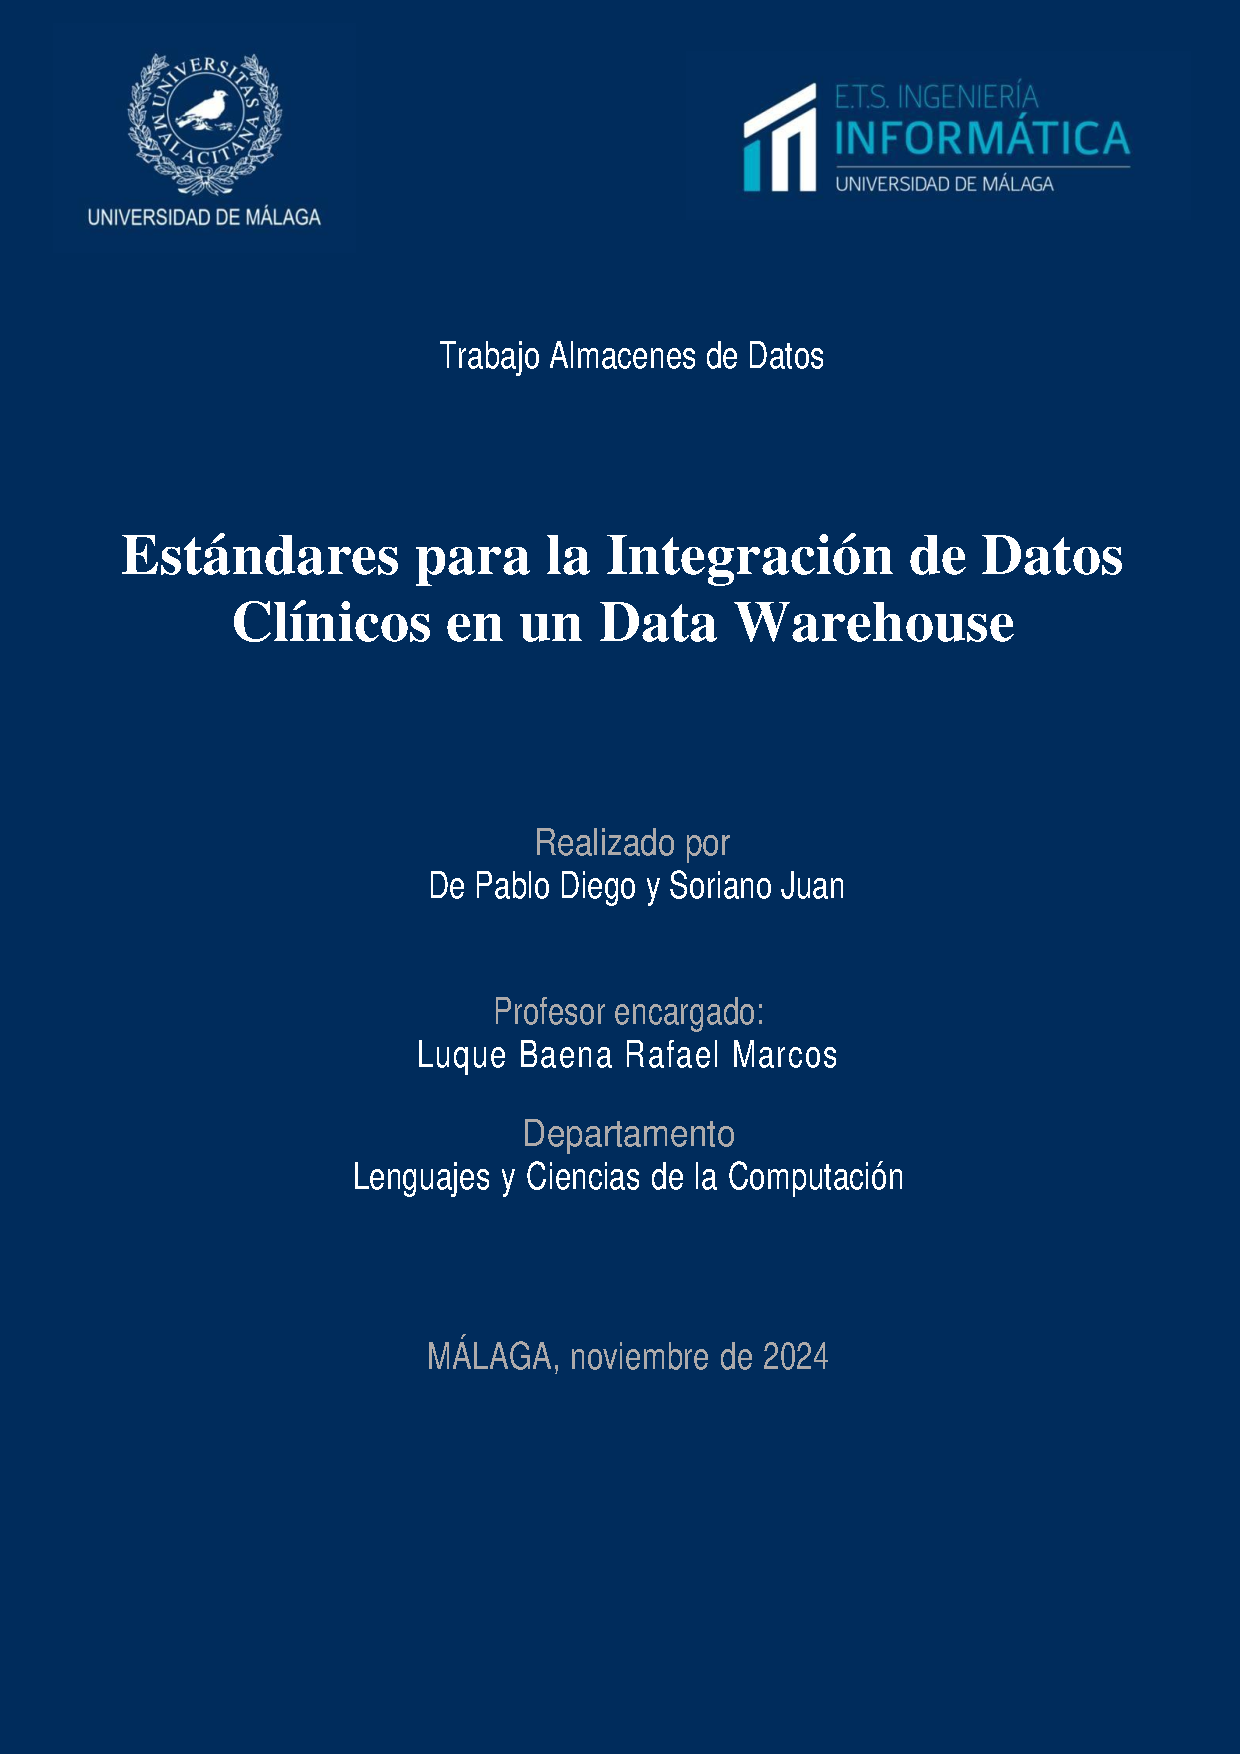
\includepdf[noautoscale=true, width=\paperwidth]{cover.pdf}
	
	%% Title
	\clearpage
	\setcounter{page}{1}
	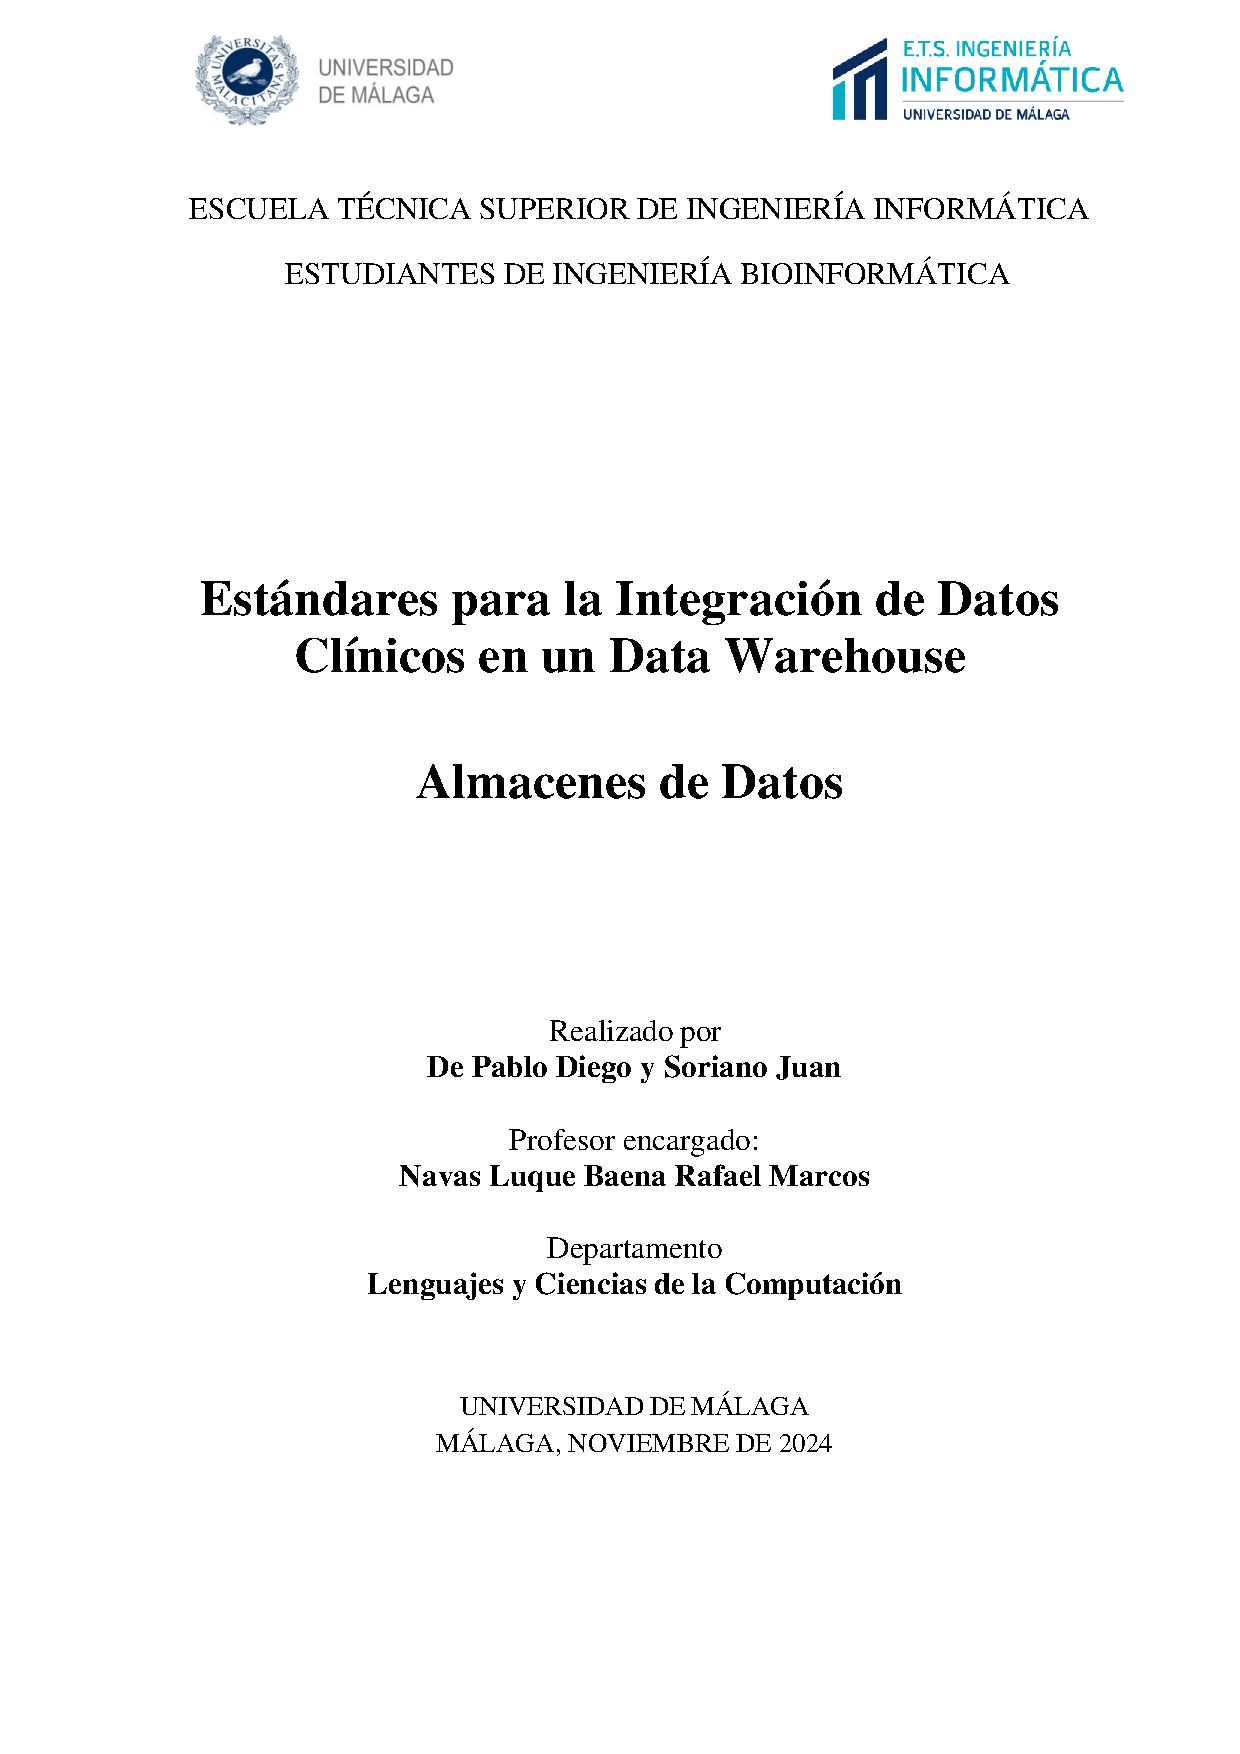
\includepdf[noautoscale=true, width=\paperwidth]{title.pdf}
	
	%%%%%%%%%%%%%%%%%%%%%%%%%%%%%%%%%%%%%%%%%%%%%%%%%%%%%%%%%%%%%%%%%%%%%%%%%%%
	
	% Índice automático
	\tableofcontents
	\newpage
	
	% Sections
	\section{Introducción a la Integración de Datos Clínicos en un Data Warehouse}
	
	La integración de datos clínicos en un warehouse es fundamental para la centralización, normalización y accesibilidad de datos clínicos provenientes de diversas fuentes en un único repositorio  \cite{founderzDW}\cite{asteraHealthcareData}.
	
	La complejidad de integrar datos clínicos radica en la diversidad de los sistemas y formatos utilizados por las diferentes organizaciones de salud, como hospitales, laboratorios, y clínicas especializadas\cite{revistaMedicaManejoInformacion}. Con el fin de proponer una solución para este problema, se desarrollaron frameworks de interoperabilidad, como HL7, FHIR, SNOMED CT y LOINC, que permiten estructurar la información para su correcta integración en un data warehouse\cite{meditecsInteroperabilidad}. Este proceso asegura que los datos almacenados se mantengan consistentes y precisos\cite{founderzDW}.
	
	El objetivo de este trabajo es analizar cómo se estandariza la información para la integración de datos clínicos en un data warehouse, herramientas utilizadas, y el impacto de esta tecnología en la gestión y uso de la información de salud.
	
	
	\section{Fundamentos y Conceptos Clave de los Data Warehouses en el Ámbito Clínico}
	
	Un \textbf{data warehouse} (almacén de datos) es un sistema diseñado para la recolección, almacenamiento y análisis de grandes volúmenes de datos provenientes de diversas fuentes. Esta plataforma reúne diversas tecnologías y componentes aprovechando al máximo los datos. Permite almacenar una gran cantidad de datos, así como también su tratamiento y análisis. El objetivo es \textbf{transformar los datos brutos en informaciones útiles}, y volverlos disponibles y accesibles para los usuarios \cite{Portal2017}.
	
	La función de un data warehouse es actuar como un repositorio centralizado donde se recopilan datos de múltiples fuentes, como bases de datos transaccionales, sistemas ERP o archivos externos. Estos datos pueden ser estructurados (tablas relacionales), semiestructurados (como archivos XML o JSON) o no estructurados (texto libre, imágenes)\cite{Portal2017}.
	
	Una vez los datos llegan al data warehouse, pasan por un proceso de \textbf{ETL} (Extracción, Transformación y Carga), donde son limpiados, organizados y transformados para su análisis. Los usuarios pueden acceder a estos datos mediante herramientas de \textbf{Business Intelligence} (BI), consultas SQL o visualizaciones interactivas.
	
	Al centralizar la información, las organizaciones obtienen una visión completa y coherente de sus datos, lo que facilita la toma de decisiones basadas en hechos. Además, el data warehouse habilita técnicas de \textbf{data mining}, que permiten descubrir patrones ocultos y tendencias para mejorar estrategias comerciales o de operación\cite{kimball2013}.
	
	En el ámbito clínico, los \textbf{sistemas de información sanitaria} (SIS) recopilan volúmenes crecientes de datos provenientes de la atención médica rutinaria. Esta fuente de \textbf{datos del mundo real} (RWD, por sus siglas en inglés) ofrece un gran potencial para mejorar la calidad de la atención médica. Por un lado, estos datos aportan beneficios directos al paciente —usos primarios— al ser fundamentales para el desarrollo de la medicina personalizada. Al mismo tiempo, brindan beneficios indirectos —usos secundarios— al acelerar y mejorar la generación de conocimiento sobre patologías, condiciones de uso de productos y tecnologías sanitarias, así como la evaluación de su seguridad, eficacia y utilidad en la práctica diaria. Estos datos también son útiles para medir el impacto organizacional de las tecnologías de salud. El \textbf{manejo eficiente de grandes volúmenes de datos} a través de un data warehouse es una de las ventajas más importantes que permite maximizar el uso de esta información para mejorar los resultados en salud.
	
	
	\subsection{Fases del Flujo de Datos en un Clinical Data Warehouse (CDW)}
	
	El \textbf{Clinical Data Warehouse (CDW)} es una infraestructura que permite consolidar datos provenientes de uno o varios \textbf{Sistemas de Información Médica} (HIS, por sus siglas en inglés) en formatos homogéneos, independientemente del marco organizativo o del origen de los datos. Esta estructura es esencial para facilitar la reutilización de la información en diversos contextos como la gestión, la investigación y la atención médica. \cite{doutreligne2023}
	
	La \textbf{Figura \ref{fig:Flujo}} ilustra las cuatro fases clave del flujo de datos que conforman un CDW, desde la recopilación de las fuentes originales hasta los usos finales, destacando el proceso de transformación e integración de los datos.
	
	\begin{figure}[h!]
		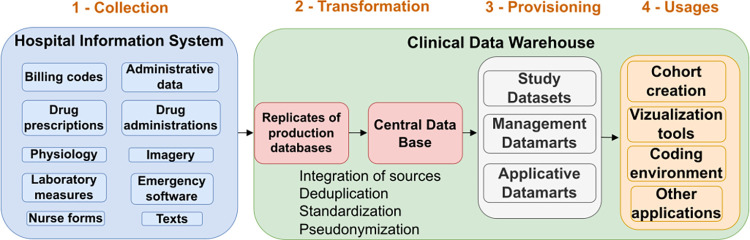
\includegraphics[width=1\textwidth]{image/Flujo.jpg}
		\caption{Cuatro pasos del flujo de datos del Sistema de Información Hospitalaria: (1) recopilación, (2) transformaciones y (3) aprovisionamiento. CDW, almacén de datos clínicos.\cite{doutreligne2023}}
		\label{fig:Flujo}
	\end{figure}
	
	\begin{enumerate}
		\item \textbf{Recopilación (Collection)}  
		La primera fase consiste en extraer los datos de las distintas fuentes que componen el HIS. Estas fuentes pueden incluir datos administrativos, prescripciones de medicamentos, mediciones fisiológicas, resultados de laboratorio, formularios de enfermería, entre otros. El objetivo principal es capturar la mayor variedad de datos posibles para que el CDW sirva como un repositorio central que refleje de manera precisa la información clínica almacenada en los sistemas hospitalarios. Cada una de estas fuentes puede estar almacenada en diferentes formatos, lo que subraya la necesidad de normalización en las fases posteriores.
		
		\item \textbf{Transformación (Transformation)}  
		Tras la recopilación, los datos pasan por un proceso de transformación donde se integran y armonizan para asegurar su coherencia. En esta fase se distinguen varias etapas clave:  
		\begin{itemize}
			\item \textit{Integración de fuentes}: Los datos de diferentes bases son unificados en una base central.  
			\item \textit{Desduplicación de identificadores}: Se eliminan las duplicaciones y se normalizan los identificadores que se puedan repetir en diversas fuentes.  
			\item \textit{Estandarización}: Un modelo de datos único, independiente de los sistemas de origen, asegura que los datos se almacenen y estructuren bajo un esquema común. Este proceso es crucial para asegurar la interoperabilidad y puede incluir la adopción de nomenclaturas estándar como SNOMED CT o LOINC.  
			\item \textit{Pseudonimización}: Con el fin de proteger la privacidad del paciente, los datos sensibles son anonimizados mediante técnicas de pseudonimización, eliminando o codificando cualquier información directamente identificativa.
		\end{itemize}
		
		\item \textbf{Provisión (Provisioning)}  
		Una vez que los datos han sido transformados, se almacenan en una base central y se dividen en subconjuntos específicos o \textit{datamarts}, que permiten su reutilización tanto en usos primarios como secundarios. Estos \textit{datamarts} pueden estar orientados a diferentes objetivos, como estudios específicos, gestión administrativa o aplicaciones clínicas. El uso de \textit{datamarts} especializados optimiza el acceso a los datos y facilita la creación de \textit{cohortes}, la utilización de \textit{herramientas de visualización}, así como el acceso a un \textit{entorno de codificación} y otras aplicaciones.
		
		\item \textbf{Usos (Usages)}  
		En esta última fase, los usuarios del CDW pueden acceder a los datos ya procesados y almacenados en los \textit{datamarts} a través de aplicaciones y herramientas especializadas. Los principales usos incluyen:
		\begin{itemize}
			\item \textit{Creación de cohortes}: Selección de subpoblaciones específicas basadas en criterios clínicos para su análisis en estudios de investigación.  
			\item \textit{Herramientas de visualización}: Plataformas que permiten explorar los datos mediante gráficos, tablas y otras representaciones visuales para facilitar el análisis.  
			\item \textit{Entornos de codificación}: Espacios diseñados para realizar análisis avanzados y procesar los datos de manera eficiente mediante técnicas de \textit{machine learning} o análisis estadístico.  
			\item \textit{Otras aplicaciones}: Los datos también pueden ser reutilizados en diversas aplicaciones, desde la mejora de procesos clínicos hasta la evaluación de nuevas tecnologías o tratamientos.
		\end{itemize}
	\end{enumerate}
	
	
	
	
	
	\section{Estándares de Interoperabilidad en Datos Clínicos}
	
	
	El aspecto más importante de los estándares de integración de datos clínicos es la interoperabilidad para la integración efectiva en un data warehouse, ya que permite que sistemas de salud, que a menudo operan de forma independiente, puedan compartir información coherente y confiable. \cite{meditecsInteroperabilidad}
	Permite a los profesionales de la salud y a los investigadores disponer de un acceso centralizado a la información, independientemente de las plataformas o sistemas en los que se generaron originalmente los datos.\cite{meditecsInteroperabilidad}
	Detallaremos los estándares de integración más utilizados:
	
	
	\subsection{Estándares de mensajería y estructura de datos:}
	
	Hay varias formas de estructurar la información:
	
	\subsubsection{HL7 (Health Level 7)} 
	HL7 es uno de los estándares de interoperabilidad más utilizados en el ámbito clínico. Desarrollado por la organización Health Level Seven International. Permite el intercambio de datos entre aplicaciones de salud mediante mensajes estandarizados que contienen información crítica, como datos de pacientes, resultados de laboratorio y diagnósticos médicos. Es ampliamente adoptado en sistemas de salud debido a su capacidad para manejar grandes volúmenes de datos de forma eficaz. 
	
	
	\textbf{Ejemplo de Uso de HL7:} Un hospital necesita compartir los resultados de laboratorio de un paciente con su proveedor de atención primaria. Utilizando HL7, los resultados de laboratorio se codifican en un mensaje HL7 que contiene los campos de información relevantes, como la identificación del paciente, el tipo de prueba realizada y los resultados numéricos de la prueba.
	
	Un mensaje HL7 típico, con el estándar HL7 V2, podría tener un formato similar a este\cite{meditecsHL7}:
	
	\begin{verbatim}
		MSH|^~\&|LABSYSTEM|HOSPITAL|CLINIC|12345|202410261230||ORU^R01|123|P|2.3
		PID|1||123456^^^HOSPITAL^MR||Doe^John||19650215|M||2106-3^White^HL70005
		OBR|1|12345|67890|CBC^Complete Blood Count^HL70001|202410261200|||||||
		OBX|1|NM|59462-2^Hemoglobin^LN||13.5|g/dL|13.5-17.5|N|F
		OBX|2|NM|718-7^White Blood Cell Count^LN||6.8|x10^3/uL|4.5-11.0|N|F
	\end{verbatim}
	
	
	
	En este mensaje:
	\begin{itemize}
		\item MSH es el segmento de encabezado del mensaje.
		\item PID contiene la información del paciente.
		\item OBR y OBX detallan el tipo de prueba y los resultados obtenidos.
	\end{itemize}
	
	Este mensaje HL7 se envía al sistema del proveedor de atención primaria, quien recibe los datos y los integra en el expediente médico del paciente de forma automatizada, permitiendo así una consulta rápida y eficiente en cualquier momento.
	
	
	\subsubsection{FHIR (Fast Healthcare Interoperability Resources)} 
	
	FHIR es un estándar relativamente nuevo y es considerado la evolución de HL7. Diseñado por la misma organización que HL7, FHIR permite el intercambio de datos rápido y seguro utilizando formatos ás utilizados como JSON y XML. La modularidad de FHIR, a través de recursos (resources) individuales que representan entidades clínicas, como pacientes, observaciones, y procedimientos, facilita la integración de distintos tipos de datos clínicos., Permite que sistemas diversos accedan a datos precisos y estructurados en tiempo real, lo que es ideal para aplicaciones web y móviles.
	En esta página (https://www.hl7.org/fhir/resourcelist.html) se puede encontrar que campos son necesarios dependiendo de nuestras necesidades. 
	
	\begin{figure}[h!]
		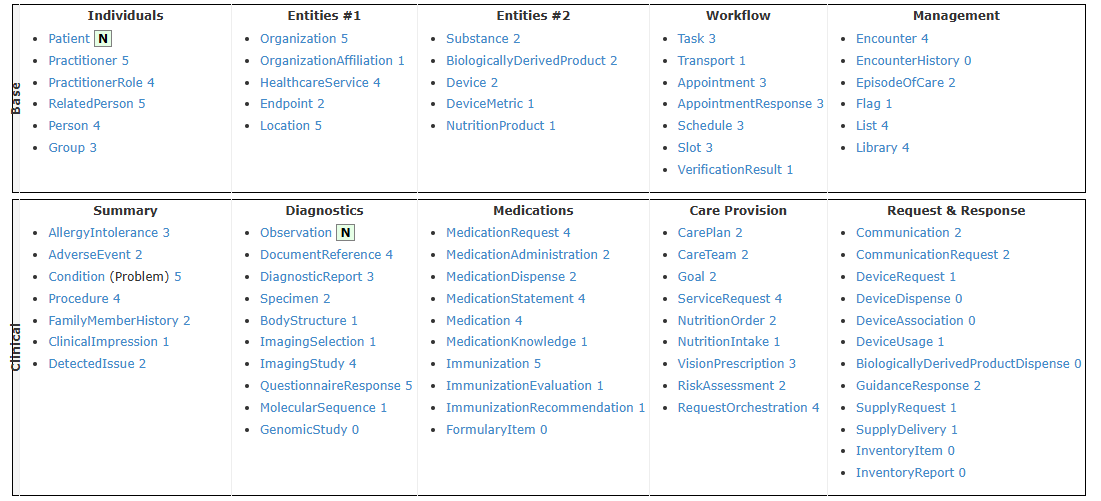
\includegraphics[width=1\textwidth]{image/1.png}
		\caption{Recursos de FHIR}
		\label{fig:1}
	\end{figure}
	\vspace{9cm}
	
	\textbf{Ejemplo de Uso de FHIR:} Imaginemos una aplicación móvil que permite a los pacientes visualizar su historial médico. Utilizando FHIR, la aplicación puede solicitar datos específicos al sistema de EHR (Electronic Health Record) del hospital en tiempo real.
	
	Si quisiéramos transferir un paciente de un hospital a otro, sería necesario que el json, que contiene la información del paciente tuviera algunos de los campos especificados en la imagen:
	\vspace{1cm}
	
	\begin{figure}[h!]
		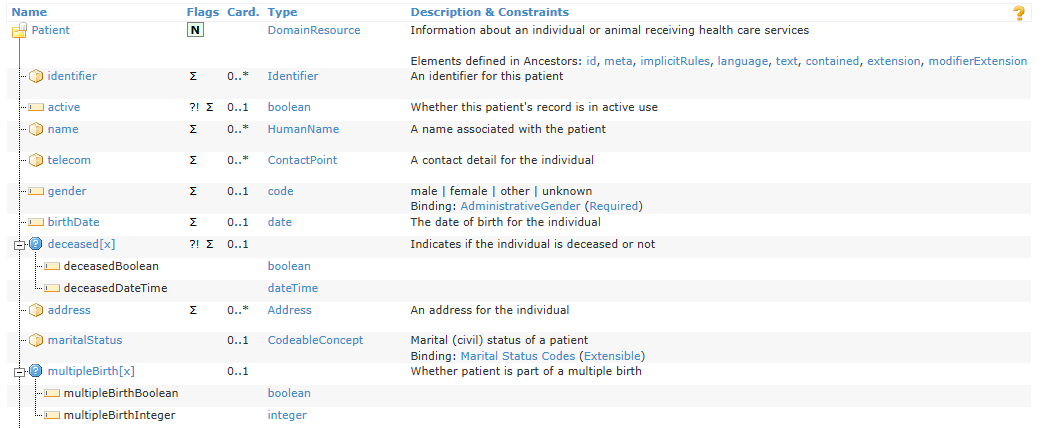
\includegraphics[width=1\textwidth]{image/2.png}
		\caption{Campos de Paciente}
		\label{fig:2}
	\end{figure}
	
	
	Un recurso FHIR en JSON para obtener la información de un paciente podría verse así:
	
	\begin{verbatim}
		{
			"resourceType": "Patient",
			"id": "123",
			"identifier": [
			{
				"use": "usual",
				"system": "http://hospital.org/patient",
				"value": "12345"
			}
			],
			"name": [
			{
				"use": "official",
				"family": "Doe",
				"given": [
				"John"
				]
			}
			],
			"gender": "male",
			"birthDate": "1965-02-15"
		}
	\end{verbatim}
	
	Hay otros recursos como Observation (resultados de laboratorio) o MedicationRequest (ver recetas).
	
	\subsection{Estándares de codificación de términos:}
	
	Estos estándares funcionan para estandarizar los datos de diagnóstico de enfermedades y síntomas, entre otros, mediante su codificación.
	
	\subsubsection{SNOMED CT}
	
	SNOMED CT (Systematized Nomenclature of Medicine Clinical Terms) se utiliza para codificar términos clínicos de manera uniforme. Permiten describir con precisión diagnósticos, procedimientos, síntomas y otros datos clínicos en un formato estandarizado. Al usar SNOMED CT, se asegura que los términos médicos sean interpretables por diferentes sistemas y usuarios en diversas regiones y entornos \cite{sanidadSNOMEDCT}.
	
	\textbf{Ejemplo de Uso de SNOMED CT:} Un médico registra el diagnóstico de un paciente en su expediente electrónico, indicando que tiene diabetes tipo 2. En lugar de escribir “diabetes tipo 2” de forma libre, el sistema de EHR convierte este diagnóstico en un código SNOMED CT específico, como 44054006, que representa “diabetes mellitus tipo 2”\cite{bioportalSNOMEDCT}.
	
	Al registrar el diagnóstico con el código SNOMED CT:
	
	\begin{itemize}
		\item Los sistemas pueden realizar búsquedas de manera uniforme; por ejemplo, todos los pacientes con 44054006 pueden ser agrupados para analizar estadísticas de prevalencia.
		
		\item Los profesionales médicos en distintas instituciones entienden el diagnóstico sin importar el idioma o variaciones regionales, ya que el código es único y universal.
		
		\item Permite realizar análisis de datos clínicos sobre enfermedades, tratamientos y evolución de pacientes, basados en términos clínicos estandarizados y consistentes.
	\end{itemize}
	
	\subsubsection{LOINC}
	
	LOINC es un estándar utilizado principalmente para codificar resultados de laboratorio y observaciones clínicas. Cada prueba de laboratorio y observación tiene un código único en LOINC que permite compararlos de forma consistente entre distintas instituciones de salud. Esto es especialmente útil cuando los datos se centralizan en un data warehouse y se necesita comparar resultados de laboratorio obtenidos en diferentes lugares o con diferentes equipos \cite{meditecsInteroperabilidad}.
	
	Ejemplo de Uso de LOINC: Un laboratorio realiza un análisis de glucosa en sangre y obtiene un valor de 105 mg/dL. El resultado se codifica con el código LOINC 2345-7, que representa una “Glucosa en suero o plasma”\cite{loinc2345}.
	
	
	El uso de LOINC permite que:
	\begin{itemize}
		\item Los resultados de glucosa en sangre se almacenan en un data warehouse con el mismo código LOINC, sin importar el hospital o laboratorio que haya realizado la prueba.
		
		\item Al realizar consultas y comparaciones en el data warehouse, todos los valores de glucosa se identifican por el mismo código 2345-7, permitiendo así obtener una visión coherente de los niveles de glucosa en diferentes pacientes o en el mismo paciente a lo largo del tiempo.
		
		\item Por ejemplo, al analizar el historial de un paciente con el código 2345-7, es posible ver la evolución de su glucosa en sangre y evaluar si ha habido mejoría o empeoramiento en sus niveles. Esto puede ayudar a ajustar tratamientos y realizar diagnósticos más precisos.
	\end{itemize}
	
	
	
	\section{Arquitectura del Data Warehouse Clínico}
	
	La arquitectura de un \textbf{data warehouse clínico} es fundamental para el análisis de datos de salud. Esta arquitectura se compone de varias capas que interactúan entre sí para garantizar que los datos sean accesibles, confiables y utilizables para la toma de decisiones clínicas. A continuación, se explican las capas y los componentes esenciales de esta arquitectura.\cite{ESIC_DataWarehouse}
	
	\subsection{Capas de la Arquitectura del Data Warehouse}
	
	La \textbf{Figura \ref{fig:Arqui}} ilustra una simplificación de la arquitectura típica de un data warehouse clínico se puede dividir en las siguientes capas:
	
	
	\begin{figure}[h!]
		\centering % Acentúa la figura al centro
		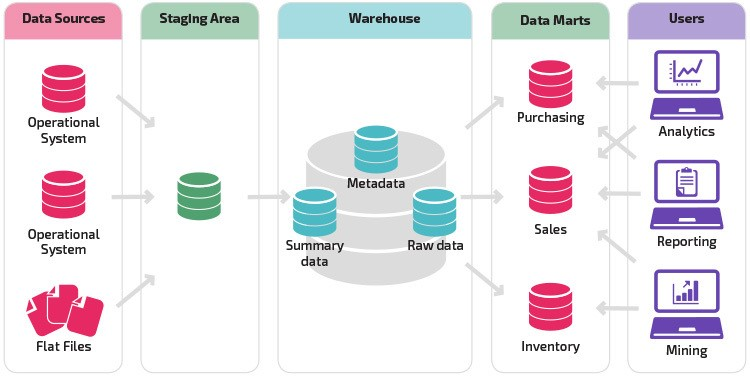
\includegraphics[width=1\textwidth]{image/Arquitectura.jpg}
		\caption{5 puntos de la arquitectura del Data Warehouse: (1) Fuentes de Datos, (2) Carga (ETL), (3) Warehouse o almacenamiento, (4) Procesamiento y (5) Presentación.} % Asegúrate de cerrar el caption correctamente
		\label{fig:Arqui}
	\end{figure}
	\vspace{9cm}
	
	\begin{itemize}
		\item \textbf{Capa de Fuentes de Datos:} Esta es la base del data warehouse y está compuesta por diversas fuentes de datos clínicas, como lo pueden ser:
		\begin{itemize}
			\item \textit{Registros Electrónicos de Salud (EHR):} Documentos digitales que contienen información sobre la salud de los pacientes.
			\item \textit{Sistemas de Información de Salud (HIS):} Plataformas que integran y gestionan datos clínicos y administrativos.
			\item \textit{Sistemas de Laboratorio:} Sistemas que gestionan datos de pruebas y resultados de laboratorio.
			\item \textit{Dispositivos de Monitoreo:} Equipos que recogen datos de salud en tiempo real, como monitores de signos vitales.
		\end{itemize}
		
		\item \textbf{Capa de Extracción, Transformación y Carga (ETL):} Esta capa es crucial para preparar los datos antes de ser almacenados en el data warehouse. Las actividades incluyen:
		\begin{itemize}
			\item \textit{Extracción:} Obtención de datos desde las diferentes fuentes mencionadas.
			\item \textit{Transformación:} Normalización, limpieza y enriquecimiento de datos para asegurar la calidad y consistencia. Esto puede incluir la conversión de formatos, eliminación de duplicados y la integración de datos de distintas fuentes.
			\item \textit{Carga:} Inserción de los datos transformados en el repositorio del data warehouse.
		\end{itemize}
		
		\item \textbf{Capa de Almacenamiento:} En esta capa se encuentran los datos organizados y estructurados, donde se utilizan diferentes modelos de datos:
		\begin{itemize}
			\item \textit{Modelo Estrella:} Un esquema que organiza los datos en una tabla de hechos central conectada a varias tablas de dimensiones. Este modelo facilita consultas rápidas y análisis.
			\item \textit{Modelo Copo de Nieve:} Una variante del modelo estrella, donde las tablas de dimensiones están normalizadas para reducir la redundancia de datos.
			\item \textit{Data Mart:} Subconjuntos de un data warehouse que están diseñados para un área específica, como el manejo de enfermedades crónicas o análisis de laboratorio.
		\end{itemize}
		
		\item \textbf{Capa de Procesamiento:} Esta capa se encarga de procesar y analizar los datos almacenados. Se puede incluir:
		\begin{itemize}
			\item \textit{Minería de Datos:} Técnicas que permiten descubrir patrones, correlaciones y tendencias en grandes volúmenes de datos clínicos.
			\item \textit{Análisis Predictivo:} Modelos estadísticos y algoritmos que utilizan datos históricos para predecir eventos futuros, como la probabilidad de enfermedades.
			\item \textit{Informes y Dashboards:} Herramientas que permiten a los usuarios visualizar datos y métricas a través de gráficos interactivos y resúmenes visuales.
		\end{itemize}
		
		\item \textbf{Capa de Presentación:} Esta capa proporciona acceso a los datos a los usuarios finales. Los usuarios pueden interactuar con los datos a través de:
		\begin{itemize}
			\item \textit{Interfaces de Usuario:} Aplicaciones web o móviles que permiten a los profesionales de la salud consultar y analizar datos de manera intuitiva.
			\item \textit{Herramientas de BI (Business Intelligence):} Software que ayuda en la toma de decisiones a través de la creación de informes, análisis de tendencias y generación de métricas de rendimiento.
		\end{itemize}
	\end{itemize}
	
	
	Además de la arquitectura, también se deben considerar otros componentes clave para asegurar la calidad y eficiencia de un data warehouse clínico. Esto incluye la gobernanza de datos, que establece políticas para garantizar la calidad y privacidad de la información; la gestión de calidad de datos, que utiliza herramientas para asegurar la precisión y completitud de los datos mediante limpieza y monitoreo; la seguridad de datos, que protege la confidencialidad e integridad de la información a través de autenticación y cifrado; la interoperabilidad, que permite el intercambio efectivo de datos entre sistemas mediante estándares como HL7 y FHIR; y el mantenimiento y soporte, que asegura la continuidad operativa mediante actualizaciones y soporte técnico.\cite{Portal2017}
	
	
	\section{Proceso ETL para la Integración de Datos Clínicos}
	Explica las etapas de Extracción, Transformación y Carga (ETL) para normalizar y consolidar datos clínicos de diversas fuentes.
	La integración de datos clínicos en un data warehouse requiere de un proceso ETL (Extracción, Transformación y Carga) robusto que pueda manejar la heterogeneidad de las fuentes de datos y normalizar la información para su análisis y uso posterior.
	
	\subsection{Extracción}
	La etapa de extracción implica la recolección de datos desde múltiples fuentes heterogéneas, como sistemas de gestión hospitalaria (HIS), sistemas de registros médicos electrónicos (EHR), sistemas de laboratorio, y bases de datos de farmacia. Estas fuentes suelen tener estructuras de datos diferentes y utilizar estándares específicos, como HL7 o FHIR, y muchas veces incluso formatos propietarios\cite{keepcodingExtraccion}.
	Extracción en Datos Clínicos:
	\begin{itemize}
		\item \textbf{Acceso a fuentes variadas:} Conectar con diferentes sistemas, incluyendo sistemas de registros médicos electrónicos, dispositivos médicos y aplicaciones clínicas.
		
		\item \textbf{Acceso seguro:} Asegurar que la extracción de datos cumpla con las normativas de privacidad de datos de salud (como HIPAA en EE. UU. \cite{fbiHIPAA} o GDPR en Europa \cite{comisionEUDataProtection}).
		
		\item \textbf{Manejo de formatos de datos:} Leer e interpretar formatos como XML, JSON, y mensajes HL7 V2, o FHIR, así como datos de bases de datos SQL y archivos CSV.
	\end{itemize}
	
	\textbf{Ejemplo de Extracción en Datos Clínicos:} Un sistema de EHR contiene información de consultas médicas de pacientes en formato HL7. Para extraer esta información, el proceso ETL se conecta con el sistema de EHR mediante una interfaz segura y descarga los datos en formato HL7 V2 para luego proceder con la transformación.
	
	\subsection{Transformación}
	La transformación es la etapa más complicada del proceso ETL. Implica la normalización y estandarización de los datos extraídos. Los datos clínicos suelen estar codificados en diferentes sistemas (ej., SNOMED CT, LOINC, ICD-10) \cite{KeepCodingFaseTransformacion}.El objetivo principal será convertir estos datos en un formato común que permita su análisis conjunto. Esta etapa incluye varios subprocesos clave:
	\begin{itemize}
		\item \textbf{Estandarización de formatos:} Convertir los datos a un formato común, como JSON o CSV, y unificar estructuras y tipos de datos.\cite{AsteraDataStandardization}. 
		
		\item \textbf{Normalización y limpieza de datos:} Corregir valores inconsistentes, eliminar duplicados y manejar valores nulos o faltantes. \cite{DatosMaestrosLimpiezaDatos}
		
		\item \textbf{Codificación:} Mapear términos médicos a un estándar de codificación unificado, como SNOMED CT para diagnósticos y LOINC para resultados de laboratorio. \cite{ITDOSNOMEDCT}
		
		\item \textbf{Integración de datos:} Combinar datos de distintas fuentes en una estructura unificada, lo que puede implicar el mapeo de distintos campos de datos al mismo campo en el data warehouse.
	\end{itemize}
	
	\textbf{Ejemplo de Transformación en Datos Clínicos:} Imaginemos que se tienen registros de diferentes laboratorios en formatos y códigos distintos. Algunos laboratorios usan términos de texto libre para describir las pruebas de laboratorio, mientras que otros utilizan LOINC. En la fase de transformación, el proceso ETL asigna códigos LOINC a las pruebas descritas en texto libre y convierte todos los registros a un mismo formato de archivo (ej., JSON o CSV) para que puedan ser integrados en el data warehouse.
	
	Además, durante esta etapa, los datos de un paciente con identificadores distintos en cada sistema fuente se unen mediante un identificador único (como el número de historia clínica o ID de paciente en el hospital), consolidando así el historial del paciente.
	
	
	\subsection{Carga}
	
	La etapa de carga implica mover los datos transformados y normalizados al data warehouse clínico, donde estarán disponibles para el análisis y consulta. En esta fase, se deben considerar aspectos como la frecuencia de actualización de los datos, el diseño del modelo de datos en el data warehouse, y el control de calidad.
	
	Tipos de Carga:
	\begin{itemize}
		\item \textbf{Carga completa:} La primera vez que se cargan los datos al data warehouse, se hace de manera completa, es decir, se carga todo el histórico de datos clínicos\cite{ESIC_DataWarehouse}.
		
		\item \textbf{Carga incremental:} Para actualizaciones periódicas, solo se cargan los datos nuevos o los que hayan sido modificados desde la última carga, optimizando el uso de recursos y el tiempo de carga. \cite{ESIC_DataWarehouse}.
	\end{itemize}
	
	\textbf{Ejemplo de Carga en Datos Clínicos:} Una vez que los registros de laboratorio han sido transformados y estandarizados, se insertan en el data warehouse en tablas relacionadas con los datos clínicos del paciente, como en una tabla de “Pruebas de Laboratorio”. El sistema puede configurarse para realizar cargas incrementales diarias, de forma que cualquier nuevo resultado de laboratorio se agregue automáticamente al data warehouse, permitiendo a los analistas y médicos consultar la información más reciente.
	
	
	\section{Beneficios de la Integración de Estándares  Datos Clínicos}
	
	La integración de datos clínicos a través de un \textit{Data Warehouse} clínico ofrece múltiples beneficios para el manejo de la información sanitaria que han sido mencionadas anteriormente. Al centralizar los datos de diversas fuentes y garantizar su interoperabilidad mediante estándares como HL7 o FHIR, se facilita el acceso a información precisa y en tiempo real. Esto permite a los médicos y gestores de salud tomar decisiones más informadas y basadas en hechos, lo que mejora directamente la calidad de la atención. El uso de datos integrados también acelera la capacidad de realizar análisis avanzados, permitiendo a los sistemas de salud anticiparse a complicaciones, identificar tendencias en tiempo real y planificar de manera más eficiente los recursos sanitarios.
	
	Además, los \textit{Data Warehouses clínicos} ayudan a la investigación médica y el cumplimiento normativo. Al consolidar grandes volúmenes de datos en un formato estandarizado, los investigadores pueden realizar estudios más robustos, como análisis epidemiológicos o ensayos clínicos, que no solo apoyan la investigación científica sino que también permiten descubrir patrones que podrían mejorar las prácticas médicas. Asimismo, la capacidad de cumplir con las normativas y generar informes precisos para entidades regulatorias o aseguradoras se ve facilitada, promoviendo una mayor transparencia y control de calidad en la prestación de servicios médicos.
	
	
	\section{Relación con el Curso de Almacenes de Datos}
	
	Durante el curso se ha proporcionado una base sólida sobre el manejo, diseño y uso de \textit{data warehouses}. Muchos de los conceptos aplicados en este trabajo, como la estructura multidimensional y los procesos ETL, están fundamentados en los conocimientos adquiridos en clase. Hemos aprendido a diferenciar entre los sistemas de bases de datos transaccionales (OLTP) y los almacenes de datos (OLAP), entendiendo cómo el cambio de paradigma, que se enfoca en agregar datos en lugar de actualizarlos o eliminarlos, permite crear una visión histórica completa. Esta visión es esencial en sistemas clínicos, donde el mantenimiento del historial íntegro de los datos de los pacientes es clave para mejorar el análisis, apoyar en la toma de decisiones, y avanzar en el cuidado de la salud.
	
	La experiencia de trabajar con \textit{data warehouses} durante el curso nos ha mostrado su relevancia directa en el ámbito de la salud. Aplicar técnicas como la extracción, transformación y carga (ETL) sobre datos clínicos reales permite a los ingenieros en salud centralizar y estructurar información médica de manera eficiente. Esto no solo facilita el análisis predictivo y la identificación de patrones en grandes volúmenes de datos clínicos, sino que también permite diseñar soluciones más efectivas para optimizar recursos en hospitales y mejorar el manejo de pacientes. Lo que en clase se aborda desde una perspectiva técnica, en el contexto clínico se traduce en herramientas que impactan directamente la calidad de la atención médica y la investigación científica.
	
	
	\section{Ejemplos-Demo de Uso de Integración de Datos Clínicos con Estándares}
	
	
	\subsection{Ejemplo con estándar  FHIR:}
	En este caso lo que intentaremos es postear la información de un paciente con el estándar de datos FHIR en formato JSON en un servidor de  FHIR.
	
	\subsubsection{Extracción y Transformación}
	Dado que partimos de un json y el servidor de FHIR trabaja con formato json, no hace falta transformarlo.
	
	Primero necesitamos crear un archivo recurso FHIR y un json que cumpla con los estándares de mensaje de FHIR, por lo que para ello, primero nos descargaremos un archivo que nos ayudará a crear el json de un paciente. 
	
	Iremos al siguiente enlance nos iremos a https://hl7.org/fhir/ al apartado de documentación y le daremos a Downloads - Schemas, Code, Tools (https://hl7.org/fhir/downloads.html) y nos descargaremos un zip (https://hl7.org/fhir/fhir.schema.json.zip), que contiene un fhir.schema.json con toda la información del estándar de FHIR sobre cómo crear un json.
	
	Creamos un setting.json, que se relacione con el json descargado: 
	
	\begin{figure}[h!]
		\centering
		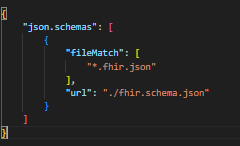
\includegraphics[width=0.8\textwidth]{image/3.png}
		\caption{settings.json}
		\label{fig:3}
	\end{figure}
	
	Ahora cuando creemos un json nos aparecerán recomendaciones de los campos del estándar FHIR:
	
	\begin{figure}[h!]
		\centering
		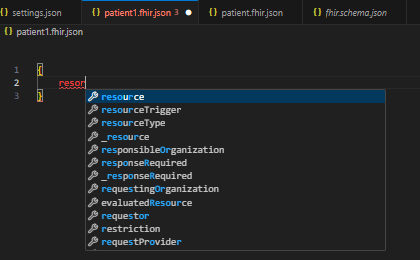
\includegraphics[width=0.8\textwidth]{image/4.png}
		\caption{VS recomienda estructuras del estándar de FHIR}
		\label{fig:4}
	\end{figure}
	\vspace{5cm}
	
	En este caso escogemos el resourceType y ponemos el valor “Patient”, ya que queremos insertar un paciente en el servidor.
	
	Después de crear el json entero siguiendo el estándar para un json de FHIR:
	\vspace{0.3cm}
	
	\begin{verbatim}
		{
			"resourceType": "Patient",
			"name": [
			{
				"use": "official",
				"given": ["Juan"],
				"family": "Soriano"
			}
			],
			"gender": "male",
			"birthDate": "2003-09-08",
			"telecom": [
			{
				"value": "987654310",
				"use": "mobile",
				"system": "phone"
			},
			{
				"system": "email",
				"value": "tornadoalert@gmail.com"
			}
			],
			"address":[
			{
				"line":[
				"213, Diamond Residency"
				],
				"city": "Málaga",
				"state": "Andalucia",
				"postalCode": "567104"
			}
			]
		}
	\end{verbatim}
	\cite{HL7Patient}
	\vspace{4cm}
	
	\subsubsection{Carga}
	
	Se dispondrá de un servidor dado por FHIR para la prueba:
	
	\begin{figure}[h!]
		\centering
		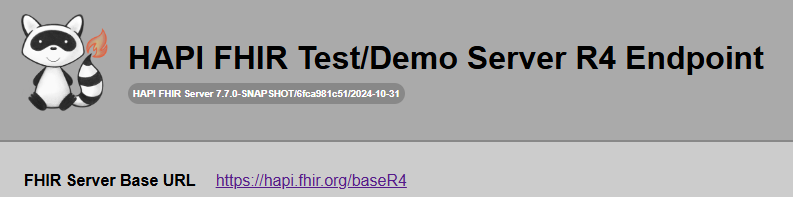
\includegraphics[width=0.8\textwidth]{image/5.png}
		\caption{Servidor de FHIR \cite{HAPI_FHIR}}
		\label{fig:5}
	\end{figure}
	
	
	Será a esta url \cite{HAPI_FHIR_Patient} a la que le lanzaremos un post para meter nuestro cliente en el servidor.
	
	Ponemos el json como cuerpo del mensaje.
	Si hacemos una petición get a https://hapi.fhir.org/baseR4/Patient/45106909, nos devolverá nuestro paciente añadido:
	
	\begin{figure}[h!]
		\centering
		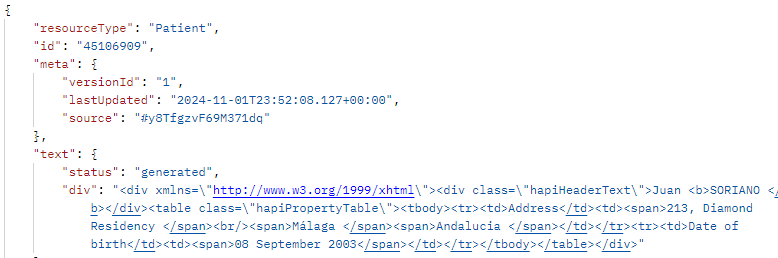
\includegraphics[width=0.8\textwidth]{image/6.png}
		\caption{Resultado de la petición get}
		\label{fig:6}
	\end{figure}
	
	Como tal no hemos integrado los datos a un datawarehouse aplicando ETL, ya que no tenemos almacenes y no hacía falta aplicar ninguna codificación de los datos, pero probamos la efectividad del estándar FHIR  para integrar datos clínicos en un repositorio único o una base de datos.
	
	\subsection{Ejemplo con estándar HL7:}
	
	Para este ejemplo utilizaremos Mirth Connect, que es una plataforma de integración de datos clínicos ampliamente utilizada en el ámbito de la salud para facilitar la interoperabilidad entre sistemas. Permite que distintos sistemas de información en salud (como EHR, HIS, LIS, y Data Warehouses clínicos) intercambien y transformen datos de manera segura y eficiente\cite{meditecsMirthConnect}. 
	Está diseñado para manejar datos en diversos formatos y estándares, como HL7, FHIR, X12, DICOM, y más, Mirth Connect permite transformar y adaptar los datos a los requisitos específicos de cada sistema, asegurando que se interpreten y utilicen de manera coherente\cite{meditecsMirthConnect}. 
	
	Mirth connect proporciona la posibilidad de crear canales para poder mandar mensajes de datos clínicos y cargarlos en un datawarehouse.
	
	En este caso, suponiendo que tenemos, ya extraída la información de un paciente siguiendo el estándar de mensajería de HL7, transformarlo y adaptar esa información, para integrarlo a una base de datos de mySQL, que simularía nuestro datawarehouse.
	
	Para el ejemplo crearemos una base de datos llamada patient, con una tabla paciente: 
	
	Haremos un query:
	
	\begin{verbatim}
		CREATE DATABASE patient; 
		USE patient;
		CREATE TABLE pacientes (
		id INT AUTO_INCREMENT PRIMARY KEY,
		nombre VARCHAR(255) NOT NULL,
		fecha_admision DATETIME NOT NULL,
		diagnostico VARCHAR(255)
		);
	\end{verbatim}
	
	\begin{figure}[h!]
		\centering
		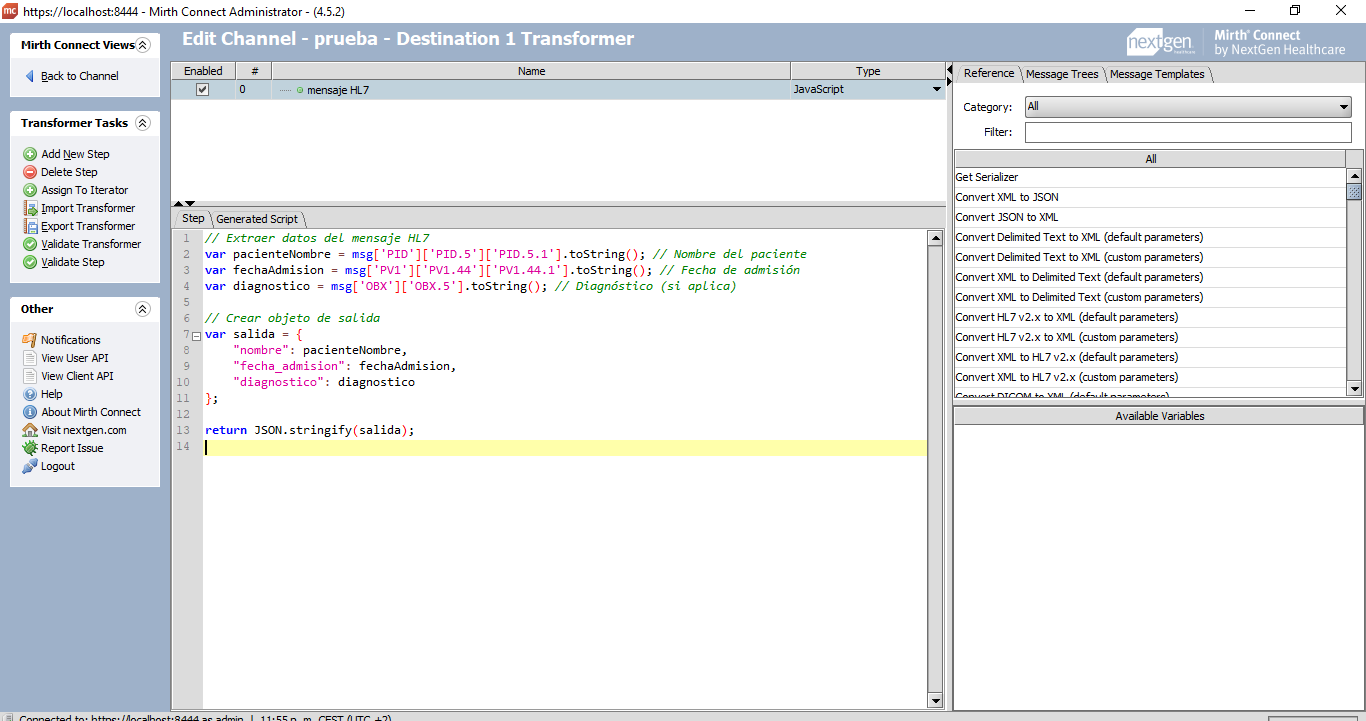
\includegraphics[width=0.8\textwidth]{image/7.png}
		\caption{Script para feedback}
		\label{fig:7}
	\end{figure}
	
	\subsubsection{Fase de extracción y transformación}
	
	Este es el msg template utilizado con el estándar de HL7:
	
	\begin{verbatim}
		MSH|^~\&|SendingApplication|SendingFacility|ReceivingApplication|ReceivingFacility|202310261200||ADT^A01|123456|P|2.5
		EVN|A01|202310261200
		PID|1||123456^^^Hospital^MR||Doe^John^||19800101|M|||
		PV1|1|I|WardA^Room101^Hospital|U|1|1234^Smith^Jane^^Dr.| | | | |202310261200|
		OBX|1|CE|DIAG^Diagnóstico||Hipertensión Arterial|||F
	\end{verbatim}

	Con este msg template, estamos avisando al canal que por él, mandaremos mensajes HL7 con esa estructura. 
	
	\subsubsection{Transformer HL7:}
	El transformador nos ayudará a captar la información que nos interesa del mensaje HL7, y adaptarla a nuestra base de datos mySQL. Esta transformación se llevará a cabo mediante el siguiente script de java:
	\begin{verbatim}[language=JAVA]
		// Extraer datos del mensaje HL7
		var pacienteNombre = msg['PID']['PID.5']['PID.5.2'].toString(); 
		var diagnostico = msg['OBX']['OBX.5']['OBX.5.1'].toString();
		
		// Log para depuración
		logger.info('Nombre: ' + pacienteNombre);
		logger.info('Diagnóstico: ' + diagnostico);
		
		// Almacenar solo datos necesarios en un objeto temporal
		var datosParaGuardar = {
			'pacienteNombre': pacienteNombre,
			'diagnostico': diagnostico
		};
		
		// Log del objeto temporal
		logger.info("Datos para guardar: " + JSON.stringify(datosParaGuardar));
		
		// Almacenar los datos extraídos en msg
		msg['pacienteNombre'] = pacienteNombre;
		msg['diagnostico'] = diagnostico;
		
		\subsubsection{Crear variables:}
		Con esta creación de variables decimos al canal, que cada vez que mandemos un mensaje, guarde como variable los siguientes campos del mensaje HL7:
		firstname
		msg['PID']['PID.5']['PID.5.2'].toString()
		diagnostico
		msg['OBX']['OBX.5']['OBX.5.1'].toString()
		
		
	\end{verbatim}
	
	\subsubsection{Carga}
	
	Configuracion de destination:
	\begin{itemize}
		\item `com.mysql.cj.jdbc.Driver`: Clase del controlador JDBC para MySQL.
		\item `jdbc:mysql://127.0.0.1:3306/patient`: URL de conexión a la base de datos MySQL.
	\end{itemize}
	
	En el script de destination, ponemos lo que se va a insertar.
	
	\begin{verbatim}
	INSERT INTO pacientes (nombre, fecha_admision, diagnostico) 
	VALUES (${nombre}, ${fecha_admision}, '${diagnostico}');
	\end{verbatim}
	
	
	
	\begin{verbatim}
	GRANT ALL PRIVILEGES ON *.* TO 'root'@'172.17.0.1' IDENTIFIED BY 'Venecia1234'
	WITH GRANT OPTION;
	FLUSH PRIVILEGES;
	ALTER USER 'root'@'%' IDENTIFIED WITH mysql_native_password BY 'NuevaContraseña';
	\end{verbatim}
	
	Ahora si enviamos a nuestro canal: 
	
	\begin{figure}[h!]
		\centering
		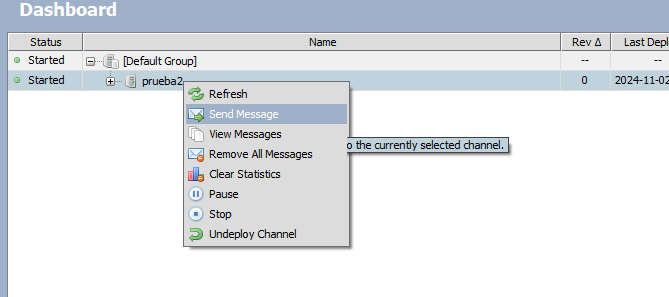
\includegraphics[width=0.8\textwidth]{image/8.png}
		\caption{Mandar mensaje al canal}
		\label{fig:8}
	\end{figure}
	
	El siguiente mensaje:
	
	\begin{figure}[h!]
		\centering
		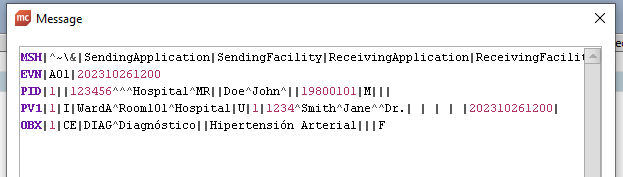
\includegraphics[width=0.8\textwidth]{image/9.png}
		\caption{Confirmación de la inserción}
		\label{fig:9}
	\end{figure}
	
	Se confirma que en efecto se han captado los campos que nos interesaban: 
	
	\begin{figure}[h!]
		\centering
		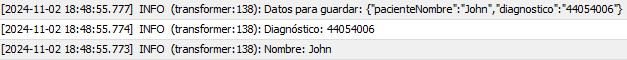
\includegraphics[width=0.8\textwidth]{image/11.png}
		\caption{Dato insertado en MySQL}
		\label{fig:11}
	\end{figure}
	
	Y como vemos queda insertado en: 
	
	\begin{figure}[h!]
		\centering
		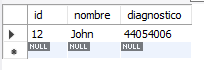
\includegraphics[width=0.5\textwidth]{image/10.png}
		\caption{Mensaje HL7}
		\label{fig:10}
	\end{figure}
	\vspace{2cm}
	
	Y como vemos queda insertado el paciente John con Diabetes tipo 2 (utilizando el estándar de codificación de diagnóstico de SNOMED CT)
	
		\section{Conclusiones y Perspectivas Futuras en la Integración de Datos Clínicos y referencias}
	
	La integración de datos clínicos en un \textit{Data Warehouse} es una solución esencial para la centralización y reutilización de grandes volúmenes de información en el ámbito de la salud. A través del uso de estándares de interoperabilidad como \textit{HL7}, \textit{FHIR}, \textit{SNOMED CT} y \textit{LOINC}, se garantiza que los datos clínicos, provenientes de diversas fuentes, sean accesibles, consistentes y útiles para la toma de decisiones. Estos estándares permiten la comunicación entre distintos sistemas y aseguran que la información se mantenga precisa y estandarizada.
	
	El diseño de un \textit{Clinical Data Warehouse} (CDW) facilita el análisis de datos históricos, lo que no solo mejora la toma de decisiones clínicas, sino que también optimiza la planificación de recursos hospitalarios y promueve la investigación médica. Las distintas capas del CDW, desde la recopilación y transformación de los datos hasta su análisis y presentación, permiten un manejo eficiente de la información, lo que resulta en una atención médica de mayor calidad y en avances en la investigación basada en datos reales.
	
	De cara al futuro, se espera que la integración de datos clínicos continúe evolucionando, facilitando un acceso aún más eficiente a información crítica para mejorar la atención médica y avanzar en la medicina personalizada. Tecnologías emergentes como la inteligencia artificial y el análisis predictivo, combinadas con el acceso centralizado a datos estructurados, prometen transformar la gestión sanitaria y la investigación en salud, permitiendo una atención más personalizada, basada en datos y optimizada para resultados clínicos.
	
	%%%%%%%%%%%%%%%%%%%%%%%%%%%%%%%%%%%%%%%%%%%%%%%%%%%%%%%%%%%%%%%%%%%%%%%%%%%
	\printbibliography
	
	
	%% Back Cover
	
\includepdf[noautoscale=true, width=\paperwidth]{backcover.pdf}
	
\end{document}